\section{Vorgehen und Datenpipeline}

TODO: 5 schritte (Best Practice) struktur-extraktion, feature-exktraktion, feature-selektion, feature-repräsentation und klassifikation \cite[Fig. 4]{yang_comprehensive_2025}

\subsection{Vorgehen}

TODO: Stichpunkte ausformulieren

% Grafik des Vorgehens

\begin{figure}[H]
    \centering
    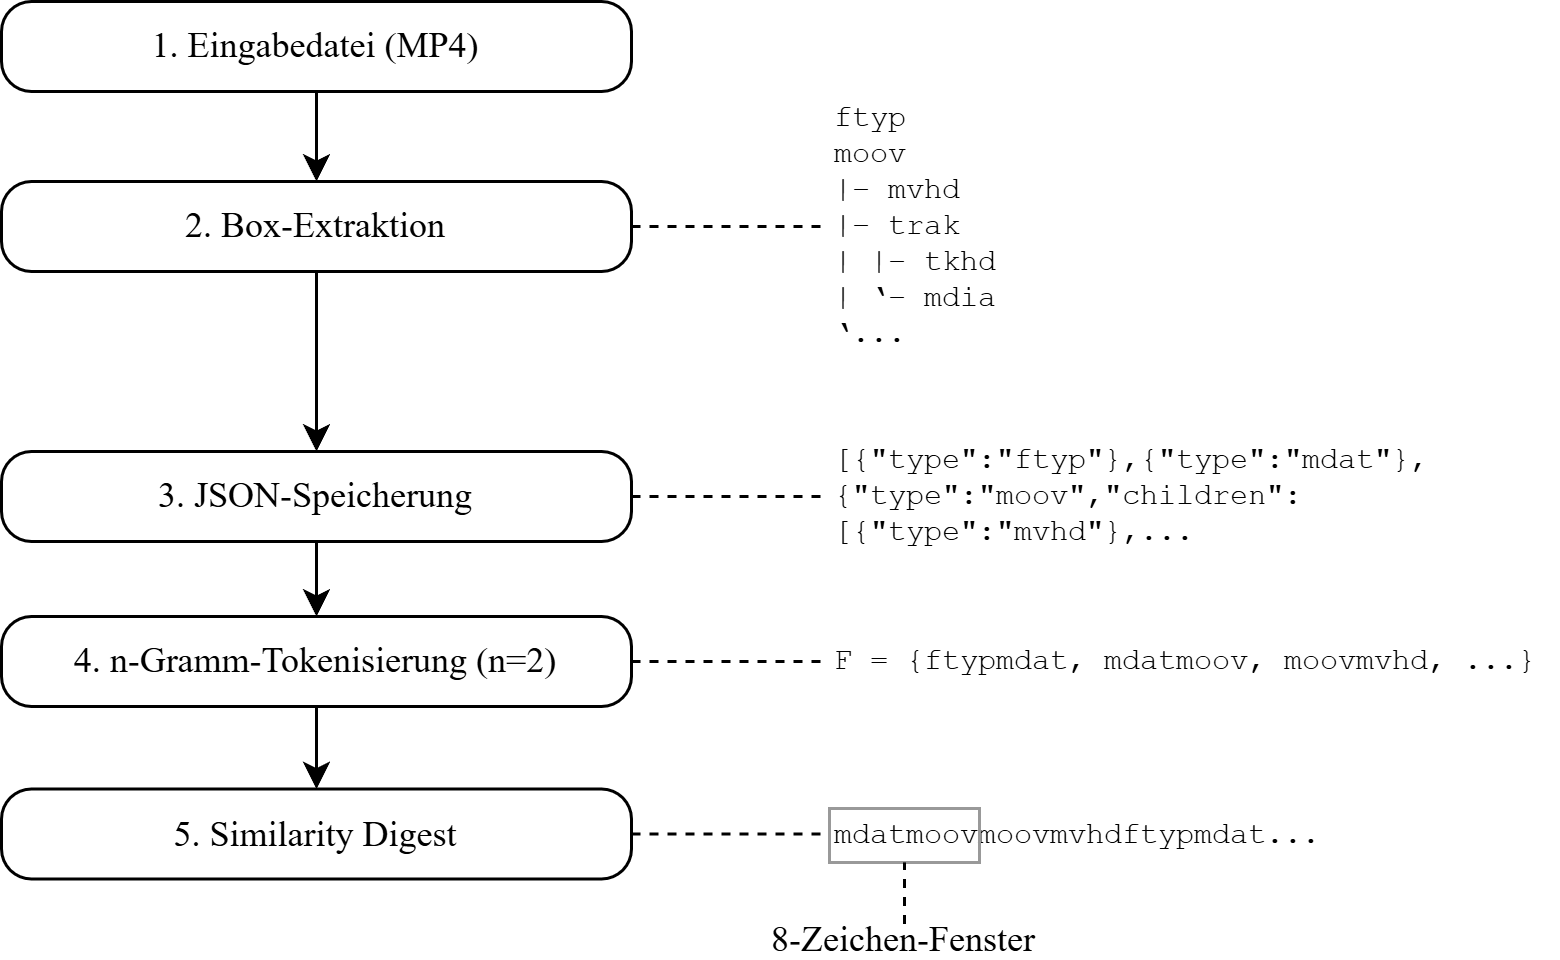
\includegraphics[width=1\linewidth]{grafiken/vorgehen-mp4.drawio.png}
    \caption{TODO: vorgehen-mp4.drawio.png}
    \label{fig:vorgehen}
\end{figure}

% Stichpunkte Vorgehen

\begin{enumerate}
    \item Mp4 Dateien parsen
    \item Box-Informationen extrahieren
    \item Box-Struktur im JSON-Format abspeichern
    \item Box-Struktur linearisieren und als 2-Gramme tokenisieren
    \item 2-Gramme als Similarity Digest abspeichern und die mit 8-Zeichen-Fenster auslesbar sind
\end{enumerate}

%%%

\newpage
\subsection{Datenpipeline}

GitHub: \url{https://github.com/lmechelk/mp4-similarity-hash/}\\

TODO: Stichpunkte ausformulieren

% BPMN der Pipeline

\begin{figure}[H]
    \centering
    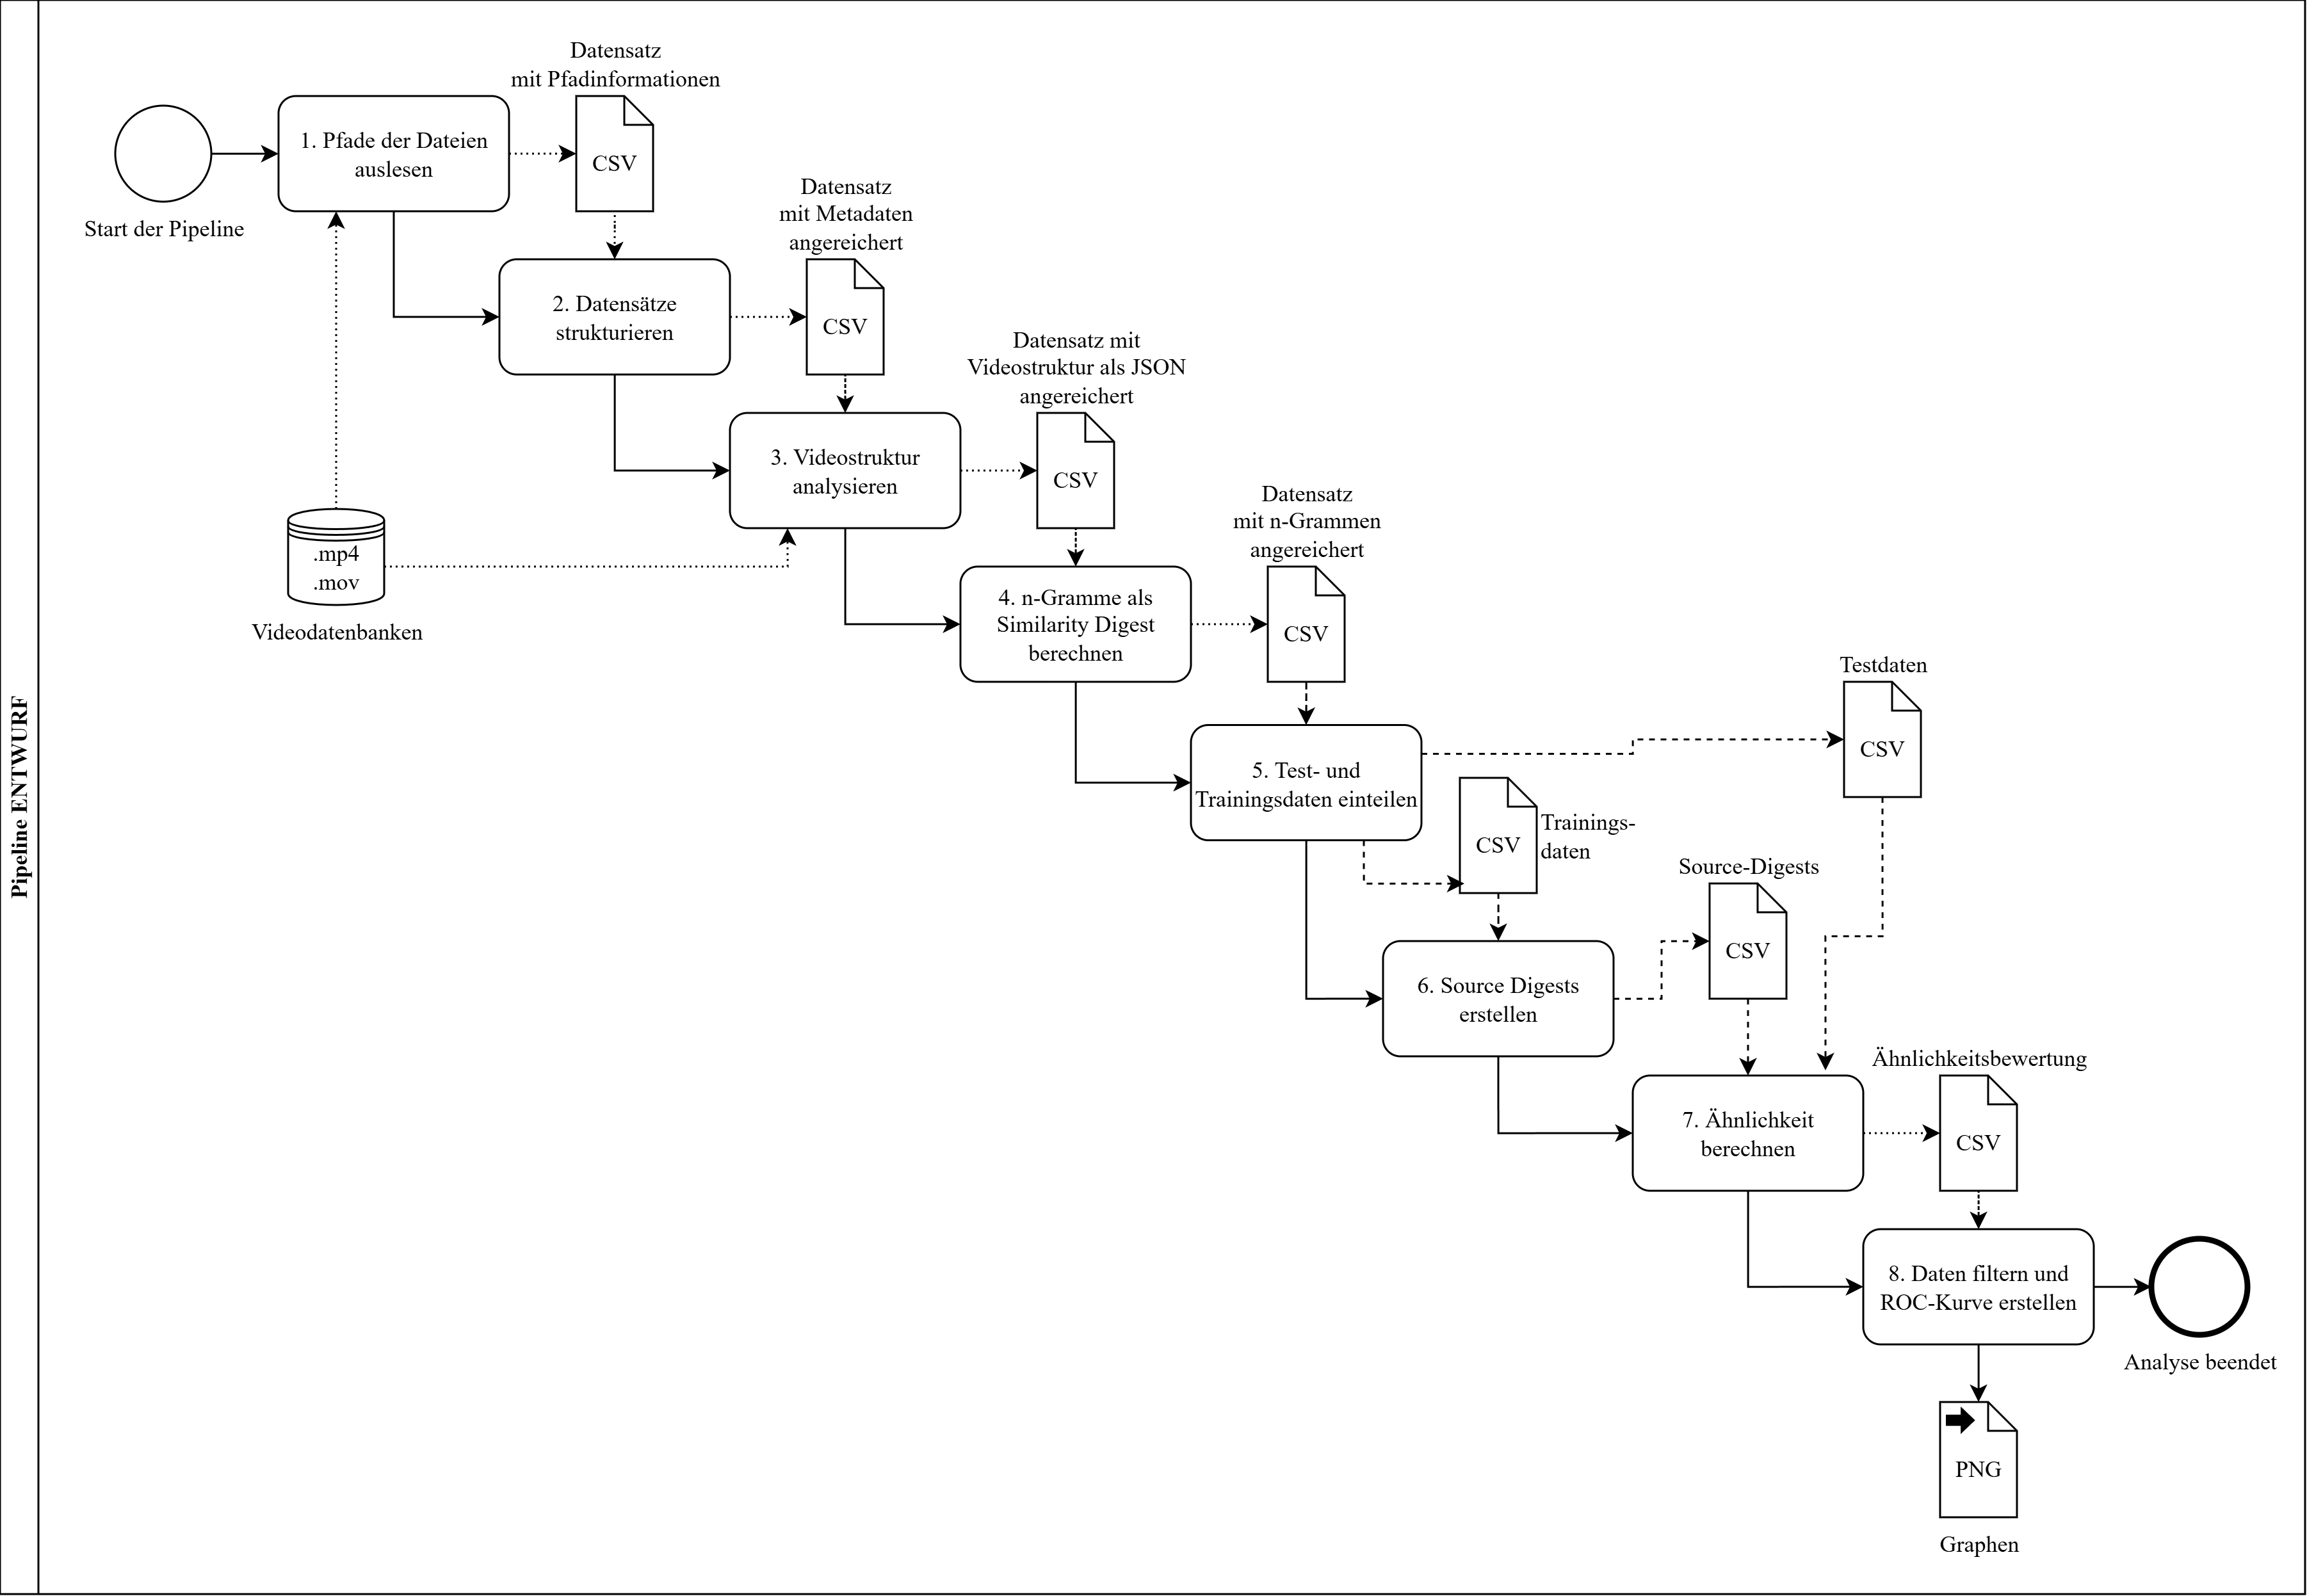
\includegraphics[width=1\linewidth]{grafiken/pipeline.drawio.png}
    \caption{TODO: pipeline.drawio.png}
    \label{fig:pipeline}
\end{figure}

% Stichpunkte Pipeline

\begin{enumerate}
    \setcounter{enumi}{-1}
    \item \textbf{Videodatenbanken bereitstellen}
    \begin{itemize}
        \item EVA-7k (5.684 Dateien)
        \item VISION (nur Videos, 1918 Dateien)
        \item eigener KI-Datensatz
    \end{itemize}
    
    \item \textbf{Pfad jeder einzelnen Videodatei auslesen}
    \begin{itemize}
        \item PATH (Dateipfad z.\,B. \url{C:/Testdaten/EVA/D01_flat_yt.mp4})
    \end{itemize}
    
    \item \textbf{Datensätze strukturieren}
    \begin{itemize}
        \item DB\_NAME (Name der Datenbank z.\,B. Vision, Eva, Selfmade)
        \item ID (Eindeutige Kennung des Geräts (\textit{Device} bei Eva/Vision) oder der AI z.\,B. D01, AI01)
        \item BRAND (Hersteller des Smartphones oder der KI z.\,B. Samsung, Grok)
        \item MODEL (Genaue Version des Smartphones oder der KI z.\,B. GalaxyS3Mini, Imagine\_0.9)
        \item MEDIA\_TYPE (Dateiendung bzw. Containerformat z.\,B. MP4, MOV)
        \item CONTENT\_SOURCE (Originäre Quelle der Videodatei, um zwischen Kameras, vollständig KI-generierten Videos mittels Text-to-Video oder Videos, die auf Bild-Vorlagen basieren (Image-to-Video), zu unterscheiden z.\,B. DIGITAL\_CAMERA, AI\_GENERATION, MIXED)
        \item CONTENT\_TYPE (Kontext der Aufnahme z.\,B. flat, indoor, outdoor, deepfake, synthetic)
        \item PROCESSING (Primäre Verarbeitung des Videos z.\,B. native, youtube, whatsapp, ai)
        \item TAMPERING (Nachträgliche Veränderung des Videos (nur Eva-DB) z.\,B. None, Avidemux)
    \end{itemize}
    
    \item \textbf{Videostruktur analysieren}
    \begin{itemize}
        \item STRUCTURE\_PRETTY (Gut lesbarer String der MP4-Struktur (nur nice to have bzw. zum Debugging) z.\,B. \texttt{moov(mvhd,trak(tkhd))})
        \item STRUCTURE\_JSON (Exakte Baumstruktur als JSON-String, der zur N-Gram-Generierung genutzt wird z.\,B. \verb|[{"type":"moov","children":[{"type":"mvhd"}]}]|)
    \end{itemize}
    
    \item \textbf{$n$-Gramme als Similarity Digest berechnen}
    \begin{itemize}
        \item NGRAM\_2 (Kompakter Similarity Digest (String), der die Signatur des Videos auf Basis von 2-Grammen (alphabetisch, duplikatbereinigt) repräsentiert; jeweils 8 lückenlose Zeichen entsprechen einem 2-Gramm-Feature z.\,B. moovmvhdtrakmvhdtraktkhd)
    \end{itemize}
    
    \item \textbf{Datensätze in Test- und Trainingsdaten einteilen}
    \begin{itemize}
        \item EVA-7k: immer die erste Datei jedes Subsets (avidemux, exiftool, \dots) aus jeder Social-Media-Kategorie (Facebook, TikTok, YouTube, \dots)
        \item VISION: immer die erste Datei jedes Content- (flat, indoor, \dots) und Processing-Types (Original, Facebook, \dots) aus jedem Device
        \item eigener KI-Datensatz: immer die erste Datei jedes KI-Modells
    \end{itemize}
    
    \item \textbf{Source-Digest erstellen}
    \begin{itemize}
        \item Digest für jede Kategorie anhand der Testdaten generieren, z.\,B. gruppiert nach Brand, Device, Social-Media, KI, KI-Modell
        \item SOURCE\_DIGEST (aggregierter Similarity Digest)
    \end{itemize}
    
    \item \textbf{Ähnlichkeit berechnen}
    \begin{itemize}
        \item GROUND\_TRUTH\_SOURCE\_DIGEST: Bezeichner für die Ground Truth, anhand der die Testdaten erstellt wurden
        \item GROUND\_TRUTH\_MP4: Bezeichner für die Ground Truth der einzelnen Test-MP4
        \item SIMILARITY: Wert von 0 bis 1 gem. Tversky-Berechnung (kein Penalty bei fehlenden Boxen in Testdatei, Penalty bei zusätzlichen Boxen in Testdatei)
    \end{itemize}
    
    \item \textbf{Daten filtern und auswerten}
    \begin{itemize}
        \item ROC und AUC berechnen
        \item Graphen erstellen
    \end{itemize}
\end{enumerate}

\begin{table}[htbp]
    \centering
    \resizebox{\textwidth}{!}{%
    \begin{tabular}{lllllllllll}
        \toprule
        \textbf{DB\_NAME} & \textbf{ID} & \textbf{BRAND} & \textbf{MODEL} & \textbf{MEDIA\_TYPE} & \textbf{CONTENT\_SOURCE} & \textbf{CONTENT\_TYPE} & \textbf{PROCESSING} & \textbf{TAMPERING} & \textbf{STRUCTURE\_PRETTY} & \textbf{NGRAM\_2 (Auszug)} \\
        \midrule
        VISION & D15 & Apple & iPhone 6 & MOV & DIGITAL\_CAMERA & FLAT & NATIVE & NONE & \texttt{moov(mvhd,trak(tkhd))} & \texttt{moovmvhdtraktkhd} \\
        EVA-7K & D01 & Samsung & GalaxyS3Mini & MP4 & DIGITAL\_CAMERA & INDOOR & YOUTUBE & AVIDEMUX & \texttt{ftypmoov(mvhd)} & \texttt{ftypmoovmoovmvhd} \\
        SELFMADE & AI01 & Grok & Imagine\_0.9 & MP4 & AI\_GENERATION & SYNTHETIC & AI & NONE & \texttt{ftypuuidmoov(mvhd)} & \texttt{ftypuuiduuidmoov} \\
        \bottomrule
    \end{tabular}%
    }
    \caption{TODO: Beispieldatensätze}
    \label{tab:testdaten_auszug}
\end{table}

TODO: Tabelle mit Auszug der echten Datensätze
% Siehe Anhang Test mit input testdatensätze.tex